\section{Amplitude-attenuated Datasets}
\label{sec:seq}

There are a number of \ac{2D} \ac{NMR} experiments in which the
variation of a parameter in the pulse sequence leads to the generation of
\acp{FID} of the same form except for an attenuation in their amplitudes across
increments. These include experiments for the determination of translational
diffusion rates and relaxation properties such as longitudinal and transverse
decoherence rates. Here, an extension to the \ac{1D} estimation technique is
described, facilitating the determination of these properties.

\subsection{Relaxation experiments}
\label{subsec:relaxation_experiments}
Any spin system which has been perturbed from its equilibrium position will
eventually return to equilibrium by a process called
\emph{relaxation}\parencites[Chapter 5]{Cavanagh2007}{Goldman2001}{Kuprov2007}.
In many applications, two fundamental quantities are of great value: the
longitudinal relaxation rate and the transverse relaxation rate, quantified by
the times $T_1$ and  $T_2$ respectively. From a vector model perspective, $T_1$
indicates how rapidly the longitudinal component of the magnetisation vector
recovers towards equilibrium, while $T_2$ indicates the rate at which
transverse magnetisation decays to zero. Numerous factors affect these
quantities, including the rate at which the spin tumbles in space, and its
electronic environment. Well-known experiments exist to quantify both of these
quantities.

\note{PS figure}

\subsubsection{Measuring $T_1$: Inversion recovery}
\label{subsec:invrec}
The inversion recovery experiment involves the simple pulse sequence $\ang{180}
\rightarrow \tau \rightarrow \ang{90} \rightarrow \tone$. The initial
\ang{180} pulse inverts the magnetisation, so that it is along $-z$. During
$\tau$, the spin system undergoes longitudinal
relaxation. Finally, the \ang{90} pulse rotates the magnetisation into the
transverse plane, enabling detection. The resultant phase and magnitude of the
signal is directly related to the amount of time that longitudinal relaxation
is allowed to occur. With $\tau = \qty{0}{\second}$, a signal with
maximal amplitude, but a phase of \ang{180} will result. At the other extreme of
very long $\tau$, the spin system will have reverted
back to equilibrium, such that a signal which also has maximal amplitude, but a
phase of \ang{0} will be realised. By sequentially adjusting $\tau$ in a
\ac{2D} experiment, a series of spectra will be obtained in which the intensity
of each peak will vary according to
\begin{equation}
    a\left(\tau\right) = a_{\infty} \left( 1 - 2 \exp\left( -\frac{\tau}{T_1}\right) \right),
\end{equation}
where $a_{\infty}$ is the intensity of the peak acquired when the spin system
has returned to equilibrium.


\subsubsection{Measuring $T_2$: \acs{CPMG}}
\label{subsec:cpmg}
In an analogous fashion to the inversion recovery experiment, by creating
transverse magnetisation and leaving it to evolve for different amounts of
time, it is possible to determine $T_2$. This might lead one to believe
that the pulse sequence $\ang{90} \rightarrow \tau \rightarrow \tone$ would be
effective for  $T_2$ determination. However the presence of J-modulation would
generate undesirable spectra with phase-modulated peaks. As well as this the presence of field inhomogeneities will cause relaxation at a faster rate than anticipated, which is incorporated in the quantity $T_2^*$. The effects of
J-modulation and field inhomogeneity can be nullified if rapid refocussing is
applied, by subjecting the spin system to a train of spin echoes. The classic
route to $T_2$ measurement is the \ac{CPMG}
experiment\cite{Carr1954,Meiboom1958}, comprising $\ang{90}_x \rightarrow
\left[ \tau \rightarrow \ang{180}_y \rightarrow \tau \right]_n \rightarrow
\tone$, where the spin echo duration $\tau$ is short and fixed, and the number
of cycles $n$ can be varied to alter the total evolution time. $T_2$ attenuates
the intensity of the resulting signal according to
\begin{equation}
    a(n) = a_0 \exp\left(-\frac{2 \tau n}{T_2}\right),
\end{equation}
where $a_0$ is the intensity where no spin echo cycles were employed.

\subsection{Diffusion experiments}
\label{sec:diffusion_experiments}
\ac{NMR} is well established as a means of determining the rates of diffusion of chemical species\cite{Johnson1999,Morris2009b}.
The first showcase for determining translational diffusion coefficients came
from Stejskal and Tanner, in which they described the \ac{PGSE} pulse
sequence\cite{Stejskal1965} (Figure \ref{fig:diffusion_sequences}.a).
The \ac{PGSE} sequence consists of a conventional spin-echo ($\ang{90}
\xrightarrow{\tau} \ang{180} \xrightarrow{\tau} \text{acquire}$), with
\acp{PFG} applied after each of the \ac{RF} pulses.
As a simple overview of how the pulse sequence works, consider a single spin on
resonance with the transmitter (i.e. its rotating frame frequency is zero) in a
sample tube at position $z$ along the axis collinear with the main field.
After the \ang{90} pulse, the magnetisation will be $-M_y$.
During the first \ac{PFG}, the spin's resonance frequency will become
$\omega_{\text{PFG}} = -\gamma g z$, where $g$ is the strength of the \ac{PFG}.
Assuming the gradient is applied for a time $\delta$, the spin will
precess by an angle of  $\alpha = -\gamma g z \delta$. After the \ang{180}
pulse, the spin's magnetisation is as follows:
\[
    -M_y
    \xrightarrow{\text{PFG}} -M_y \cos(\alpha) + M_x \sin(\alpha)
    \xrightarrow{\ang{180}_y} -M_y \cos(\alpha) - M_x \sin(\alpha).
\]
Supposing that the spin has moved to a new position $z + \Delta_z$
between the end of the first gradient and the beginning of the second,
application of the second gradient causes precession by the angle
$\beta = -\gamma g (z + \Delta_z) \delta$:
\begin{equation*}
   \begin{split}
        \xrightarrow{\text{PFG}}
            &-M_y \cos(\alpha)\cos(\beta) +
            M_x \cos(\alpha)\sin(\beta) -
            M_x \sin(\alpha)\cos(\beta) -
            M_y \sin(\alpha)\sin(\beta)\\
        &= -M_y \cos(\gamma g \delta \Delta_z) -
           M_x \sin(\gamma g \delta \Delta_z),
   \end{split}
\end{equation*}
In the scenario that the spin has not translated in the $z$-direction between
\acp{PFG} ($\Delta_z = 0$), the net effect of the pulse sequence is nothing
(except for a loss of signal amplitude through $T_2$ relaxation). However, if
translation does occur, the signal phase is adjusted, as a function of the
extent of translation $\Delta_z$. The gradients have effectively been employed
to encode the change in position of the spin after a known amount of time.
Extending this idea to a system of many identical spins, which will translate
by different extents between the \acp{PFG}, individual spin contributions to
the bulk magnetisation will become dephased, leading to an attenuation of the
amplitude of the resulting FID.

\begin{figure}
   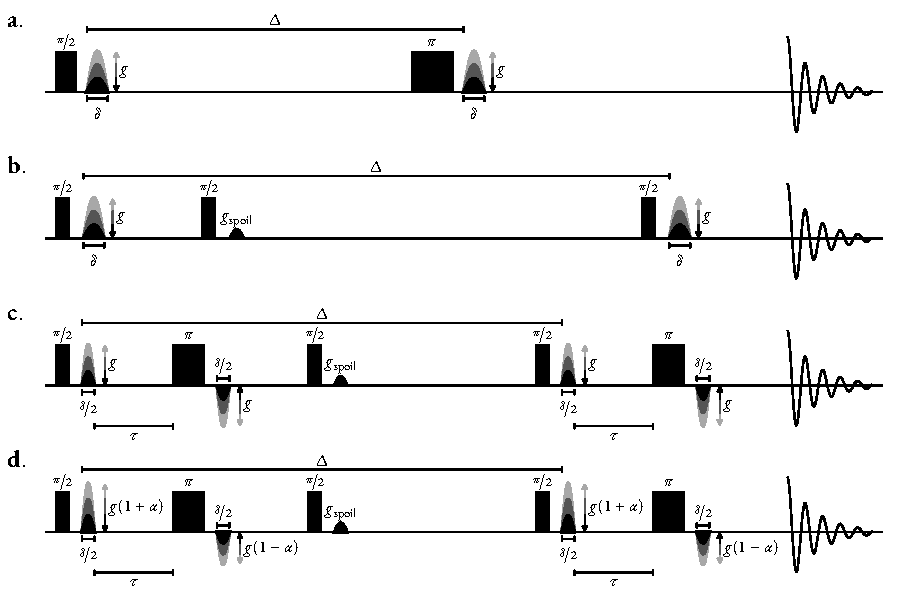
\includegraphics{diffusion_sequences/diffusion_sequences.pdf}
   \caption[
       Pulse sequences used for the determination of translational diffusion constants.
   ]{
       Pulse sequences used for the determination of translational diffusion constants.
       \textbf{a.} \acs{PGSE},
       \textbf{b.} \acs{PGSTE},
       \textbf{c.} \acs{PGSTEBP},
       \textbf{d.} One-shot DOSY.
       \ac{RF} pulses are denoted by solid rectangles. Diffusion-encoding
       gradients are denoted by sine-bell shapes with varying shades,
       indicating that the intensity is incremented to create a \ac{2D}
       dataset. Spoiler gradients are denoted by solid black sine-bell shapes.
   }
   \label{fig:diffusion_sequences}
\end{figure}

Through consideration of the Bloch-Torrey equations\cite{Torrey1956}, which
extend the classic Bloch equations to account for the effects of diffusion on
magnetisation, Stejskal and Tanner were able to derive the following equation
for the variation of the amplitude of a resonance as a function of gradient
strength, known widely as the Stejskal-Tanner equation:
\begin{equation}
    a(g) = a_0 \exp \left(- \gamma^2 \delta^2 g^2 D \left(\Delta -
    \frac{\delta}{3}\right)\right),
    \label{eq:stejskal_tanner}
\end{equation}
where
$a_0 = \lim_{g \rightarrow 0} a$,
$\gamma$ is the gyromagnetic ratio of the target nucleus
(\unit{\radian \mega\hertz\per\tesla}), \note{Should check if radians are needed}
$g$ is the gradient strength (\unit{\tesla\per\meter})\footnote{
    Gradient strengths are often expressed in units of
    \unit{\gauss\per\centi\meter}, which is equivalent to
    \qty[print-unity-mantissa = false]{e-2}{\tesla\per\meter}.
},
$\delta$ is the duration of each \ac{PFG} (\unit{\second}),
$\Delta$ is the delay between the \acp{PFG}, often known as the diffusion time
(\unit{\second}),
and $D$ is the translation diffusion constant of the species giving rise to the
resonance (\unit{\meter\squared\per\second}).
While Equation \ref{eq:stejskal_tanner} is widely stated in the literature, it is only strictly applicable when the \ac{PGSE} sequence
is used (or any other \emph{monopolar} sequence, \emph{vide infra}), and
rectangular \acp{PFG} are applied
\footnote{
    Rectangular \acp{PFG} (i.e. those in which there is an infinitesimal time
    to rise to full strength, and to fall back to zero) are in fact
    impossible to achieve as they would require gradient coils with zero
    inductance.
}.

Tanner introduced a variant of the original \ac{PGSE} experiment called
\ac{PGSTE}\cite{Tanner1970} (Figure \ref{fig:diffusion_sequences}.b). Instead
of the diffusion period including a
\ang{180} pulse, \ac{PGSTE} features two \ang{90} pulses, with the first being
applied shortly after the initial \ac{PFG}, and the second being applied just
before the second \ac{PFG}. The key difference between this and the \ac{PGSE}
experiment is that decoherence during the diffusion time is
dictated by longitudinal relaxation ($T_1$) rather than transverse relaxation
($T_2$). \ac{PGSTE} is therefore favoured in scenarios where $T_1 \ll T_2$, as
improved sensitivity is attainable.


Both \ac{PGSE} and \ac{PGSTE} employ \emph{monopolar} \acp{PFG} for diffusion
encoding, in the sense that both diffusion-encoding \acp{PFG} are polarised in a
single direction. Experiments also exist which employ
\emph{bipolar} gradient elements\cite{Cotts1989,Wu1995}, which consist of a
\ac{PFG}, followed by a \ang{180} pulse, and then a second \ac{PFG} with the
opposite polarity to the first. A well-known example is the \ac{PGSTEBP}
experiment (Figure \ref{fig:diffusion_sequences}.c). Bipolar gradient are
useful in circumstances where it is important to purge the effects of static
gradients in the sample, caused by field inhomogeneities. Morris and coworkers
have also developed the One-shot DOSY experiment\cite{Pelta2002} (Figure
\ref{fig:diffusion_sequences}.d), which requires a single transient per
gradient strength (i.e. there is no requirement for a phase-cycling scheme).
This is achieved through the use of bipolar gradients which comprise
asymmetrical \acp{PFG} with relative powers $1 + \alpha : 1 - \alpha$ for some
$ 0 > \alpha > 1$ (a common value is $0.2$).

It is virtually always the case that the amplitudes of each resonance in the
\ac{FID} abide by the following general form of the Stejskal-Tanner equation:
\begin{equation}
    a(g) = a_0 \exp\left(- c g^2 D\right)
\end{equation}
for some constant $c$ (\unit{\tesla\per\second\squared}).
It is important to note that functional form of $c$ is highly variable
dependent on the type of experiment used, and its value if affected by the
shape of the diffusion-encoding \acp{PFG}. A consideration of the Bloch-Torrey
equation for a given experiment is necessary, with an extensive overview
provided by Sinnaeve for most diffusion NMR experiments\cite{Sinnaeve2012}. In
general, $c$ is as follows:
\begin{equation}
    c = \gamma^2 \delta^2 \sigma^2 \Delta^{\prime}.
    \label{eq:stejskal_tanner_generic}
\end{equation}
$\sigma$ is the \emph{shape factor} of the \acp{PFG} (\emph{vide infra}), and
$\Delta^{\prime}$ is the effective time that diffusion is allowed to occur.
Examples of the value of $\Delta^{\prime}$ include:
\begin{subequations}
    \begin{alignat}{2}
        & \text{Monopolar gradients (\ac{PGSE}, \ac{PGSTE})} \quad && \Delta + 2 \left(\kappa - \lambda\right) \delta,
        \label{eq:monopolar}\\
        & \text{Bipolar gradients (\ac{PGSTEBP})} \quad && \Delta + \frac{\left(2 \kappa - 2 \lambda
            - 1\right)\delta}{4} - \frac{\tau}{2},\\
        & \text{One-shot}
            \quad && \Delta + \frac{\left(\kappa - \lambda\right)
            \left(\alpha^2 + 1\right) \delta}{2} +
            \frac{\left(\delta + 2 \tau\right)\left(\alpha^2 - 1\right)}{4}.
    \end{alignat}
\end{subequations}
$\tau$ is the delay between the initial \ac{PFG} and the \ang{180} pulse in
experiments with bipolar gradients.
The factors $\sigma$,  $\lambda$, and $\kappa$ are related to the shape
function $s(\epsilon) : \epsilon \in [0, 1]$ of the \ac{PFG}, which describes
the variation in the intensity of the gradient as a function of its progression.
For a rectangular gradient, $s(\epsilon) = 1 \forall \epsilon$, whereas for a
sine-bell gradient, $s(\epsilon) = \sin(\pi \epsilon)$. The cumulative
distribution of the shape function is given by:
\begin{equation}
    S(\epsilon) = \int_0^{\epsilon} s\left(\epsilon^{\prime}\right)
            \mathrm{d} \epsilon^{\prime} \quad \forall \epsilon \in [0, 1].
\end{equation}
The corresponding definition of $S$ for the case of a gradient made of discrete
steps with shape function $\symbf{s} \in \mathbb{R}^{N_g}$ is
\begin{equation}
    S\left[n\right] =
        \frac{1}{n} \sum_{i = 0}^{n} s\left[i\right] \quad
        \forall n \in \left\lbrace 0, \cdots, N_g - 1\right\rbrace,
\end{equation}
where $N_g$ is the number of points the gradient comprises. The three factors
are given by
\begin{subequations}
    \begin{gather}
        \sigma = S(1),\\
        \lambda = \frac{1}{\sigma} \int_0^1 S(\epsilon) \mathrm{d} \epsilon,\\
        \kappa = \frac{1}{\sigma^2} \int_0^1 S^2(\epsilon) \mathrm{d} \epsilon,
    \end{gather}
\end{subequations}
with their discrete counterparts being
\begin{subequations}
    \begin{gather}
        \sigma = S\left[N_g - 1\right] \\
        \lambda = \frac{1}{\sigma N_g} \sum_{n = 0}^{N_g - 1} S\left[n\right]
            = \frac{1}{\sigma N_g} \sum_{n = 0}^{N_g - 1}
            \frac{1}{n} \sum_{i=0}^{n} s\left[i\right]\\
        \kappa = \frac{1}{\sigma^2 N_g} \sum_{n = 0}^{N_g - 1} S^2\left[n\right]
            = \frac{1}{\sigma^2 N_g} \sum_{n = 0}^{N_g - 1}
            \frac{1}{n^2} \left(\sum_{i=0}^{n} s\left[i\right]\right)^2
    \end{gather}
\end{subequations}
For \acp{PFG} with a symmetrical shape, $\lambda = \nicefrac{1}{2}$. $\kappa$
is typically equal to or close to $\nicefrac{1}{3}$. It can now be seen that
Equation \ref{eq:stejskal_tanner} comes from plugging Equation
\ref{eq:monopolar} into Equation \ref{eq:stejskal_tanner_generic}, with $\sigma
= 1$,  $\lambda = \nicefrac{1}{2}$, and  $\kappa = \frac{1}{3}$. In many
situations,  $\Delta$ dominates in the expression of $\Delta^{\prime}$, and so
ensuring the correct form of $c$ could be seen as excessive. However,
especially when  $\Delta$ is not orders of magnitude greater than $\delta$, the
exact form of $\Delta^{\prime}$ used in Equation
\ref{eq:stejskal_tanner_generic} will be extremely important for accurate
measurements of $D$.

\note{Talk about means of determining $T_1$,  $D$ etc: peak pick and fit
amplitudes across increments, DOSY, DECRA/SCORE etc}

\subsection{Methodology}

\note{Give algorithm for fit of each oscillator. Include how initial guess is
generated for invrec and diffusion, and initial trust radius.}

\subsubsection{Outline of the problem}
The datasets arising from the experiments described above can be considered in
a general fashion.
Suppose the experiment of interest is run with $K \in \mathbb{N}$ increments,
such that there is a vector  $\symbf{p} \in \mathbb{R}^K$ which gives the
pulse sequence variable for each increment.
The complete dataset that results from the experiment is expected to take the
form $\symbf{Y} \in \mathbb{C}^{K \times \None}$ in which the value of the
experimental parameter attenuates the amplitudes of the contributing
resonances:
\begin{equation}
    \bY\left[k, \none\right] = \sum_{m=0}^{M-1} \symbf{A}\left[k, m\right]  \exp\left(\iu \bdphim \right)
    \exp\left(\left(2 \pi \iu \left(\bdfone_{\vphantom{\text{off}}} [m] -
    \foffone\right) - \bdetaone_{\vphantom{\text{off}}} [m] \right) \none
\Dtone\right).
\end{equation}
$\symbf{A} \in \mathbb{R}^{K \times M}$ is a matrix of the oscillator amplitudes
across the increments. A complete parameter vector for this
signal is given by $\bth \in \mathbb{R}^{(K + 3)M}$:
\begin{equation}
    \bth =
    \begin{bmatrix}
        \symbf{A}\left[0, :\right]\T \cdots & \symbf{A}\left[K-1, :\right]\T &
        \bdphi\T & \left[\bdfone\right]\T & \left[\bdetaone\right]\T
    \end{bmatrix}\T.
\end{equation}
The amplitudes are a function of the experiment parameter with the following
form:
\begin{equation}
    \symbf{A}\left[k, m\right] =
        \symbf{a}_0 \left[m\right]
        \mathcal{A} \left(
            \symbf{\psi}\left[m\right] \hspace*{2pt} | \hspace*{2pt}
            \symbf{p}\left[k\right]
        \right),
\end{equation}
where $\symbf{a}_0 \in \mathbb{R}^{M}$ is a vector of the ``maximal''
amplitudes for the oscillators, and $\symbf{\psi} \in \mathbb{R}^M$ is a vector
of the parameter of interest (diffusion coefficient, relaxation time etc.) for
each oscillator . $\symbf{a}_0 [m]$ can be thought of as the largest
possible amplitude that could be obtained for oscillator $m$ with the given
experiment:
\begin{itemize}
    \item In an inversion recovery experiment, the largest amplitude is
        achieved as $\tau \rightarrow \infty$, as the spin system will have
        returned back to equilibrium prior to the \ang{90} pulse.
    \item With \ac{CPMG} experiments, the greatest amplitude will occur when
        $n = 0$, as no time is designated for transverse
        relaxation to take place.
    \item For diffusion experiments, the largest amplitude is achieved when
        $g=0$, since no diffusion-induced dephasing of spins will have
        occurred.
\end{itemize}
The function $\mathcal{A}$ describes how the amplitudes of resonances are
attenuated by the experimental variable, and has a form which is intimately
linked to the type of experiment. For the experiments described, these forms
are provided in Table \ref{tab:seq-equations}.
\begin{table}
    \begin{center}
        \begin{tabular}{ccccccc}
            \hline
            Experiment &
            $p$ &
            $\psi$ &
            $\mathcal{A}(\psi | p)$ &
            $\frac{\partial \mathcal{A}(\psi | p)}{\partial \psi}$ &
            $\frac{\partial^2 \mathcal{A}(\psi | p)}{\partial \psi^2}$ \\ \hline
            Inversion Recovery &
            $\tau$ &
            $T_1$ &
            $\left(1 - 2 \exp \left(-\frac{\tau}{T_{1}}\right)\right)$ &
            $-\frac{2 \tau}{T_1^2} \exp\left(-\frac{\tau}{T_1}\right)$ &
            $\frac{2 \tau}{T_1^3} \exp\left(-\frac{\tau}{T_1}\right)\left(2 - \frac{\tau}{T_1}\right)$\\
            \acs{CPMG} &
            $n$ &
            $T_2$ &
            $\exp\left(-\frac{2 \tau n}{T_2}\right)$ &
            $\frac{2 \tau n}{T_2^2}\exp\left(-\frac{2 \tau n}{T_2}\right)$ &
            $\frac{2 \tau n}{T_2^3}\exp\left(-\frac{2 \tau n}{T_2}\right)
            \left( \frac{2 \tau n}{T_2} - 2 \right)$ \\
            Diffusion &
            $g$ &
            $D$ &
            $\exp\left(-c g^2 D\right)$ &
            $-c g^2 \exp\left(-c g^2 D\right)$ &
            $c^2 g^4 \exp\left(-c g^2 D\right)$ \\
            \hline
       \end{tabular}
       \caption[
           The various functional forms of $\mathcal{A}$ according to the
           different amplitude-attenuating NMR experiments considered.
       ]
       {
           The various functional forms of $\mathcal{A}$ according to the
           different amplitude-attenuating NMR experiments considered, along
           with its first and second derivatives, which are required to extract
           estimates of $\psi$ using \ac{NLP}.
       }
       \label{tab:seq-equations}
    \end{center}
\end{table}

\subsubsection{Estimating amplitude-attenuated datasets}
The close relationship between signals across increments means that completely
estimating each signal in turn is not necessary. Instead, after the first
increment is estimated from scratch, yielding $\bth_{k=0} \in \mathbb{R}^{4M}$,
the phases, frequencies and damping factors are fixed, and subsequent
increments are determined by taking the parameter estimate of the previous
iteration, and subjecting it to \ac{NLP} where only the amplitudes
are allowed to be varied. Thus, determining parameter estimates for each
iteration $k \in \lbrace1, \cdots, K-1\rbrace$ is reduced to the problem\footnote{
    $\mathcal{F}$ in \eqref{eq:fidelity-amp} reads as ``the fidelity
    with respect to the amplitudes $\bda$, given phases $\bdphi$,
    frequencies $\bdfone$, damping factors  $\bdetaone$, and \ac{FID}
    $\bY[k,:]$''. The expression has exactly the same mathematical form as
    \eqref{eq:fidelity}, though it emphasises that the phases, frequencies and
    damping factors are no longer variables to be optimised, but fixed
    parameters.
}
\begin{equation}
    \symbf{A}[k,:] = \argmin_{\bda \in \mathbb{R}^M}
        \mathcal{F}\left(\bda \hspace*{2pt} | \hspace*{2pt}
        \bdphi_{k=0}, \bdfone_{k=0}, \bdetaone_{k=0}, \bY[k,:]\right).
        \label{eq:fidelity-amp}
\end{equation}
A \ac{NLP} routine can solve this very efficiently, typically in few
iterations, on account of the linear dependence of the model with respect to
the oscillator amplitudes. The linear dependence also means that second
derivatives of the model are all zero (see \eqref{eq:amp-second-deriv}),
such that only first derivatives need to be computed to derive an exact Hessian
matrix of the fidelity.

\begin{algorithm}
    \caption[
        Routine for estimating a sequence of \ac{1D} \acsp{FID} which exhibit
        variation in amplitudes across increments.
    ]
    {
        Routine for estimating a sequence of \ac{1D} \acsp{FID} which exhibit
        variation in amplitudes across increments.
        \textsc{NLPAmp} denotes a
        routine which is akin to \textsc{NLP} (Algorithm \ref{alg:nlp}), except
        only amplitudes are allowed to be altered, whilst phases, frequencies
        and damping factors are fixed.
    }
    \label{alg:estimate-seq}
    \begin{algorithmic}[1]
        \Procedure{EstimateAmpAttenuated}{
            $\bY \in \mathbb{C}^{K \times \None},
            \symbf{r}_{\text{interest}} \in \mathbb{R}^2,
            \symbf{r}_{\text{noise}} \in \mathbb{R}^2,
            M \in \mathbb{N}_0$
        }
        \State $\bth_{0}, \symbf{\epsilon}_{0} \gets \textsc{Estimate$1$D}\left(
            \bY[0, :],
            \symbf{r}_{\text{interest}},
            \symbf{r}_{\text{noise}},
            M
            \right)
        $;
        \State $M \gets \nicefrac{\text{len}\left(\bth_0\right)}{4}$;
        \State $\bth, \symbf{\epsilon} \gets  \symbf{0} \in \mathbb{R}^{(K + 3)M}, \symbf{0} \in \mathbb{R}^{(K + 3)M}$;
        \Comment{Initialise complete parameter vector.}
        \State $\bth[:M], \symbf{\epsilon}[:M] \gets \bth_0[:M], \symbf{\epsilon}_0[:M]$;
        \Comment{Amplitudes for first increment.}
        \State $\bth[KM:], \symbf{\epsilon}[KM:] \gets \bth_0[M:], \symbf{\epsilon}_0[M:]$;
        \Comment{Phases, frequencies and damping factors, which are held constant across increments.}
        \For{$k=1, \cdots, K-1$}
            \State $\widetilde{\by} \gets \textsc{Filter$1$D}\left(
                \symbf{Y}[k,:],
                \symbf{r}_{\text{interest}},
                \symbf{r}_{\text{noise}}
                \right);
                $
            \Comment{Algorithm \ref{alg:filter-1d}.}
            \State $\bth_{k}, \symbf{\epsilon}_k \gets \textsc{NLPAmp}\left(\widetilde{\by}, \bth_{k-1}\right)$;
            \State $\bth[kM : (k+1)M], \symbf{\epsilon}[kM : (k+1)M] \gets \bth_k[:M], \symbf{\epsilon}_k[:M]$;
            \Comment{Extract amplitudes.}
        \EndFor
        \State \textbf{return} $\bth, \symbf{\epsilon}$;
        \EndProcedure
    \end{algorithmic}
\end{algorithm}

\begin{remark}
    Due to the linear dependence on amplitudes, an alternative means of
    deriving amplitudes for each increment is to determine the following
    $\forall k \in \lbrace 1, \cdots, K-1\rbrace$:
    \begin{subequations}
        \begin{gather}
            \symbf{A}[k,:] = \symbf{\Lambda}^+ \bY[k,:], \\
            \symbf{\Lambda} =
            \begin{bmatrix}
                \exp\left(\iu \bdphi [0]\right) & \cdots & \exp\left(\iu \bdphi[M-1]\right) \\
                \exp\left(\iu \bdphi [0]\right) \symbf{z}[0] & \cdots & \exp\left(\iu \bdphi[M-1]\right) \symbf{z}[M-1]\\
                \vdots & \ddots & \vdots \\
                \exp\left(\iu \bdphi [0]\right) \symbf{z}[0]^{\None-1} & \cdots & \exp\left(\iu \bdphi[M-1]\right) \symbf{z}[M-1]^{\None-1}
            \end{bmatrix},\\
            \symbf{z}[m] = \exp\left(\left(2\pi \iu \left(\bdfone[m] - \foffone\right) - \bdetaone[m]\right)\Dtone \right).
        \end{gather}
    \end{subequations}
\end{remark}


\subsubsection{Determining the parameter of interest}
Having generated a complete parameter estimate for the \ac{FID}, focus
subsequently moves to determining the parameters of interest $\symbf{\psi}$.
For each oscillator, the maximal amplitude and parameter of
interest are determined by solving the following problem $\forall m \in \lbrace
0, \cdots, M-1 \rbrace$:
\begin{equation}
    \begin{bmatrix}
        \bda_0^{(*)}[m] \\
        \symbf{\psi}^{(*)}[m]
    \end{bmatrix} =
    \argmin_{
        [a_0 \hspace*{5pt} \psi]\T \in \mathbb{R}^2
    }
    \left\lVert
        \symbf{A}[:, m] - a_0 \mathcal{A} \left(\psi \hspace*{2pt} | \hspace*{2pt} \symbf{p}\right)
    \right\rVert^2,
\end{equation}
which can also be solved using \iac{NLP} routine. The gradient vector and Hessian
matrix of the fidelity take very similar functional forms to those for \ac{FID}
estimation (see \eqref{eq:grad} and \eqref{eq:hess}), as both problems
involve solving residual sum-of-squares problems.
They are as follows $\forall i, j \in \lbrace 0, 1 \rbrace$:
\begin{subequations}
    \begin{gather}
        \symbf{g}[i] =
            -2 \left \langle
                \symbf{A}[:, m] - a_0 \mathcal{A}(\psi | \symbf{p}),
                \frac{\partial a_0 \mathcal{A} (\psi | \symbf{p})}
                {\partial \symbf{\vartheta}[i]}
            \right \rangle\\
        \symbf{H}[i,j] =
            2 \left( \left \langle
                \frac{\partial a_0 \mathcal{A} (\psi | \symbf{p})}{\partial \symbf{\vartheta}[i]},
                \frac{\partial a_0 \mathcal{A} (\psi | \symbf{p})}{\partial \symbf{\vartheta}[j]}
            \right \rangle -
            \left \langle
                \symbf{A}[:, m] - a_0 \mathcal{A}(\psi | \symbf{p}),
                \frac{\partial^2 a_0 \mathcal{A} (\psi | \symbf{p})}{\partial \symbf{\vartheta}[i]\partial \symbf{\vartheta}[j]}
            \right \rangle \right), \\
            \mathbb{R}^2 \ni \symbf{\vartheta} = [a_0 \hspace*{10pt} \psi]\T,
    \end{gather}
\end{subequations}
with explicit expressions for the requisite first and second derivatives being
\begin{subequations}
    \begin{gather}
        \frac{\partial a_0 \mathcal{A} (\psi | \symbf{p})}{\partial a_0} =
            \mathcal{A} (\psi | \symbf{p}),\\
        \frac{\partial a_0 \mathcal{A} (\psi | \symbf{p})}{\partial \psi} =
            a_0 \frac{\partial \mathcal{A} (\psi | \symbf{p})}{\partial \psi},\\
        \frac{\partial^2 a_0 \mathcal{A} (\psi | \symbf{p})}{\partial a_0^2} = 0,\\
        \frac{\partial^2 a_0 \mathcal{A} (\psi | \symbf{p})}{\partial \psi^2} =
            a_0 \frac{\partial^2 \mathcal{A} (\psi | \symbf{p})}{\partial \psi^2},\\
        \frac{\partial^2 a_0 \mathcal{A} (\psi | \symbf{p})}{\partial a_0 \partial \psi} =
            \frac{\partial^2 a_0 \mathcal{A} (\psi | \symbf{p})}{\partial \psi \partial a_0} =
            \frac{\partial \mathcal{A} (\psi | \symbf{p})}{\partial \psi}.
    \end{gather}
\end{subequations}
The functional forms of the first and second derivatives for the different
experiments of interest of $\mathcal{A}$ are given in Table
\ref{tab:seq-equations}.

\subsubsection{Displaying results}
Visualising the results from the routine described above can be done in a
similar fashion to \ac{DOSY} analysis. For each oscillator in the estimation
result, a \ac{2D} array is generated, corresponding to the outer product of the
\ac{FT} of the oscillator ($\symbf{s}_m$) and a distribution describing the
predicted value of $\psi$ ($\symbf{d}_m$).
\begin{subequations}
    \begin{gather}
        \mathbb{R}^{R \times \None} \ni \symbf{S} = \sum_{m=0}^{M-1}
        \symbf{d}_m \otimes
        \symbf{s}_m ,\label{eq:dosy-spectrum}\\
        \symbf{s}_m = \Re\left(\FT\left(\bx_m\right)\right),\\
        \bx_m\left[\none\right] = \bda_0[m] \exp\left(\iu \bdphim\right)
        \exp\left(\left(2 \pi \iu \left(\bdfonem - \foffone\right) - \bdetaonem \right) \none \Dtone\right),
    \end{gather}
    \label{eq:dosy-cross-product}
\end{subequations}
where $R \in \mathbb{N}$ is the number of samples to generate the distribution from.
The exact form that the distribution should take is not set in stone, though it
should indicate two key pieces of information:
(i) its maximum should coincide with the predicted value of $\psi$ and (ii) its
width should indicate the level of uncertainty associated with the prediction.
In this work, the
distribution used is a Gaussian distribution with mean $\symbf{\psi}[m]$ and standard
deviation $c \symbf{\epsilon}[m]$, where $\symbf{\epsilon}[m]$ is the
estimation error associated with oscillator $m$'s parameter of
interest,\footnote{
    The errors can be extracted from the Hessian matrix once the \ac{NLP}
    routine has reached convergence. See section \ref{subsec:errors} for more
    information.
}
and $c \in \mathbb{R}_{>0}$ is an arbitrary linewidth factor which can be chosen
to ensure clear visibility of the peaks.\footnote{
    In cases where the estimation error is small, the distribution can be
    so sharp relative to the resolution used for plotting, that
    $\text{max}(\symbf{d}_m)$ can be $0$ if the peak of the distribution does
    not coincide with one of the sampling values. In these situations, errors
    arise due to attempted division by $0$ (see \eqref{eq:dosy-spectrum}).
    Broadening the distribution (i.e. setting $c > 1$) resolves issues with
    plotting discrete samples.
}
\begin{subequations}
    \begin{gather}
        \symbf{d}_m\left[ r \right] = -\frac{1}{\sqrt{2 \pi (c \symbf{\epsilon}[m])^2}}
        \exp\left(
            - \frac{\left(p_r - \symbf{\psi}[m]\right)^2}{2 (c \symbf{\epsilon}[m])^2}
        \right)\quad \forall r \in \lbrace 0, \cdots, R-1 \rbrace,\\
        p_r = p_{\text{min}} + \frac{r (p_{\text{max}} - p_{\text{min}})}{R-1}.
    \end{gather}
    \label{eq:distribution}
\end{subequations}
$p_{\text{min}}$ and $p_{\text{max}}$ specify the range of values over which to
generate the distribution.

\subsection{Results}

\subsubsection{``Five multiplets''}
\begin{figure}
    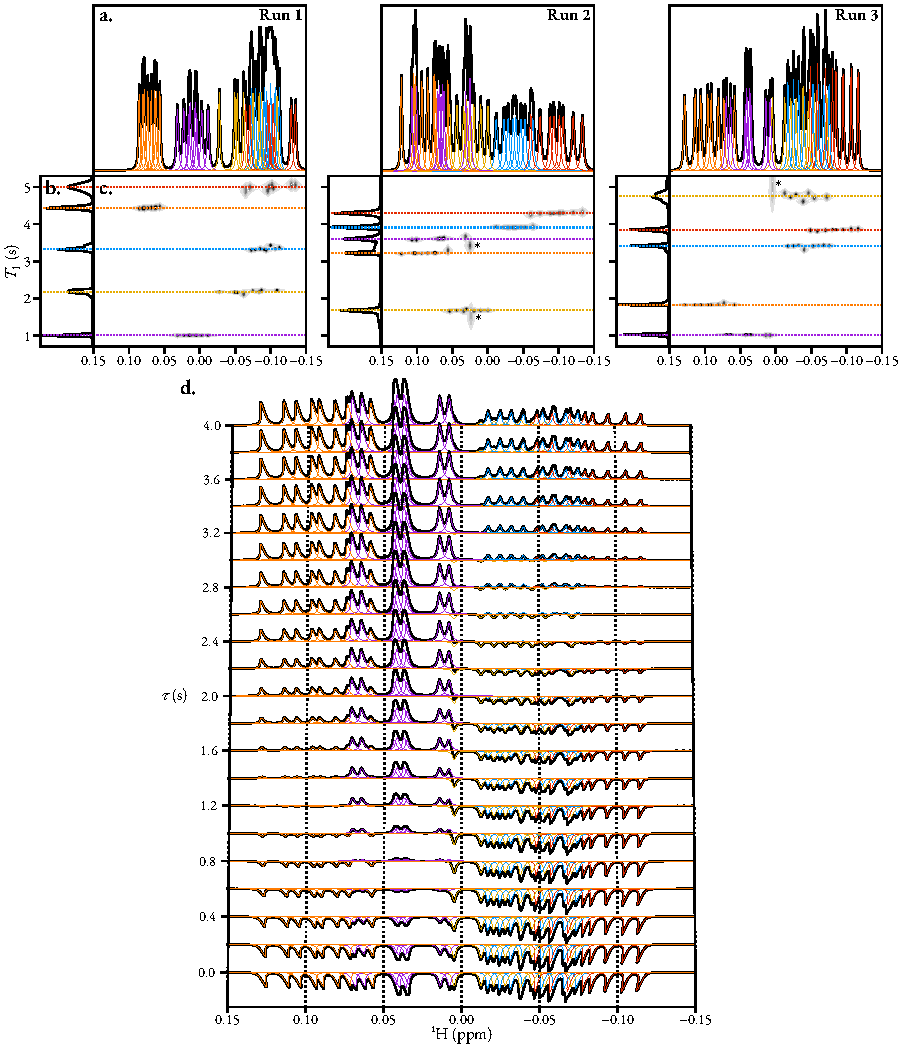
\includegraphics{five_multiplets_invrec/five_multiplets_invrec.pdf}
    \caption[
        Three examples of results generated on simulated inversion recovery
        datasets comprising five ddd multiplet structures.
    ]
    {
        Three examples of results generated on
        simulated inversion recovery datasets comprising five ddd multiplet
        structures.
        \textbf{a.} Plot of the result generated for the first increment ($\tau
        = \qty{0}{\second}$), with each plot multiplied by $-1$. Black:
        spectrum of the data. Coloured lines: spectra of individual oscillators
        generated by the estimation routine. Oscillators with the same colour
        are components of the same multiplet.
        \textbf{b.} Distribution of $T_1$ values, generated using
        \eqref{eq:distribution}, with
        $p_{\text{min}} = \qty{0.7}{\second}$,
        $p_{\text{max}} = \qty{5.3}{\second}$,
        $c = 40$,
        $R=128$.
        \textbf{c.} \ac{DOSY}-style contour plot of the result, generated using
        \eqref{eq:dosy-cross-product}.
        Dashed horizontal lines denote the true $T_1$ values for each spin.
        \textbf{c.} Estimation result for each increment for Run 3,
        illustrating the evolution of the amplitudes of each oscillator with
        $\tau$.
    }
    \label{fig:five-multiplets-invrec}
\end{figure}
Figure \ref{fig:five-multiplets-invrec} shows the result of the described
method in determining the $T_1$ values of resonances in a simulated inversion
recovery datasets featuring 5 overlapping ddd multiplet structures. The spin
systems used to generate the datasets were constructed in a similar way to that
described for the ``Four Multiplets'' example in
Section \ref{subsec:cupid-results}. In this case however, 5 estimated spins were
present instead of 4. Constraints were also placed on the shifts and
couplings to ensure that no two oscillators would have frequencies with a
difference less than $\nicefrac{\fswone}{\None}$ \note{Describe in the
appendix}. For each spin, a $T_1$ value
was sampled from $\mathcal{U}(\qty{1}{\second}, \qty{5}{\second})$, and a $T_2$
value was sampled from  $\mathcal{U}(\qty{0.2}{\second}, \qty{0.6}{\second})$.
The inversion recovery experiment was simulated using \textsc{Spinach}, with the
relaxation phenomena described by the ``extended $T_1$/$T_2$
approximation'' (see Appendix \note{REF}).
Each dataset was provided \ac{AWGN} such that the target \ac{SNR} of the
datasets as a whole was \qty{40}{\deci\bel}.
The estimation routine outlined by Algorithm \ref{alg:estimate-seq} was applied
to the generate a parameter estimate of the region which contained signals from
the estimated spins.

Despite heavy overlap between peaks, the routine was successful at
assigning each signal in the dataset with a $T_1$ value that closely agreed
with the true value (see panel b.). As is to be expected, in scenarios where
little multiplet
overlap existed, $T_1$ predictions tended to be more accurate, with smaller
associated errors (see for example the purple and orange multiplets in Run 1.
Nevertheless, adequate estimates could still be obtained in cases of severe
overlap, especially when the predicted $T_1$s for all oscillators associated
with a given multiplet are averaged. (see the red, blue and yellow multiplets
in Run 1). Particular oscillators for which the estimate of $T_1$ is
particularly far from the true value tend to be associated with large errors,
with examples denoted with an asterisk.

\subsubsection{Andrographolide Diffusion}
\note{TODO: Re-run figure generation, with sigma set to 1. Compare with dynamic
center}
\begin{sidewaysfigure}
    \centering
    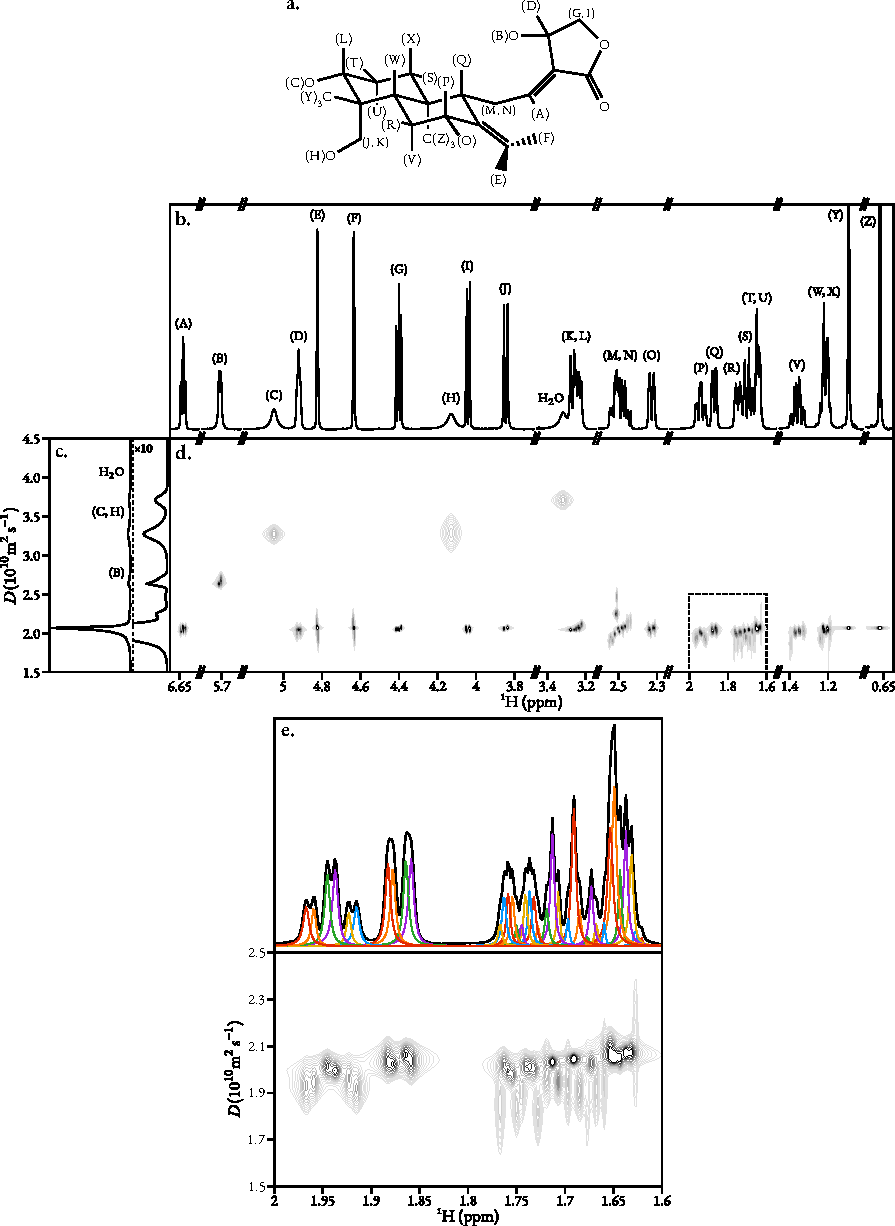
\includegraphics{andrographolide_dosy/andrographolide_dosy.pdf}
    \caption[
        Result of estimating a Oneshot \acs{DOSY} dataset of andrographolide.
    ]{
        Result of estimating a Oneshot \ac{DOSY} dataset of andrographolide in
        unfresh \ac{DMSOd6}.
        \textbf{a.} \ac{1D} spectrum.
        \textbf{b.} Diffusion profile obtained by summing the contour plot in
        c. along the $x$-axis.
        \textbf{c.} Contour plot mapping estimated oscillators to diffusion constants, with
        $p_{\text{min}} = \qty{2e-10}{\meter\squared\per\second}$,
        $p_{\text{max}} = \qty{5e-10}{\meter\squared\per\second}$,
        $c = 2.5$,
        $R=128$.
        \textbf{d.} Magnified view of the \SIrange{2}{1.6}{\partspermillion}
        spectral range, with estimated oscillator peaks plotted.
    }
    \label{fig:andrographolide-dosy}
\end{sidewaysfigure}
Figure \ref{fig:andrographolide-dosy} shows the result of applying the
estimation technique on a oneshot \ac{DOSY} dataset of andrographolide in
unfresh \acs{DMSOd6} at \qty{298}{\kelvin}. Exposure of the sample to water is
evidenced by the broad
peak around \qty{3.3}{\partspermillion}, estimated to have a diffusion constant
of \qty{4.57e-10}{\meter\squared\per\second}. On top of this, the acidic
hydroxyl protons (B, C, H) of andrographolide show significant line-broadening,
and their estimated diffusion coefficients are considerably different compared
with those of the non-hydroxyl protons, due chemical exchange with water in the
sample\cite{Chen1998}.
The diffusion profile generated suggests a diffusion constant of andrographolide of
\qty{2.54e-10}{\meter\squared\per\second}. The predicted diffusion constant for
each estimated oscillator shows decent consistency, especially with oscillators
of greater intensity. Lower intensity oscillators - especially those which
significantly overlap with other oscillators - tended to be associated with
less consistent diffusion constants and larger errors with examples of this
phenomenon apparent in panel d of the figure. A few oscillators also show a
significant deviation at around \qty{2.5}{\partspermillion}. This is likely due to
the presence of signals that make up a 1:2:3:2:1 quintet due to the presence of
partially protonated \acs{DMSO}. As the data is
insufficiently resolved to enable the separation of andrographoilde and
\ac{DMSO} signals in the estimation result, oscillators exist which
will have an amplitude profile influenced by both species, leading to an
aggregated diffusion constant. As $D_{\text{DMSO}} >
D_{\text{andrographoilide}}$, the affected oscillators show larger apparent
diffusion constants.


\subsubsection{Glucose/valine/threonine diffusion}
\note{TODO: get result from dynamic center and compare}
\begin{figure}
    \centering
    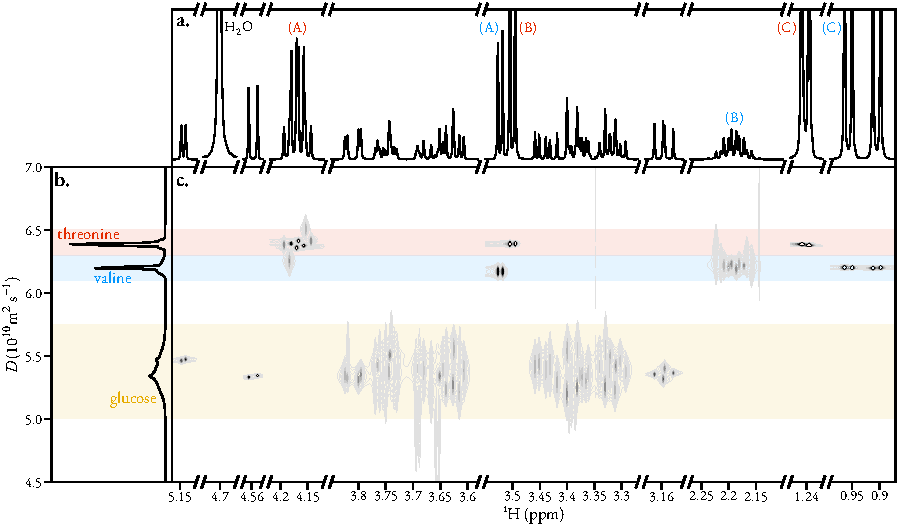
\includegraphics{glu_thre_val_diffusion/glu_thre_val_diffusion.pdf}
    \caption[
        Result of estimating a diffusion dataset for a mixture of L-threonine,
        L-valine and D-(+)-glucose.
    ]{
        Result of estimating a diffusion dataset for a mixture of L-threonine,
        L-valine and D-(+)-glucose in D\textsubscript{2}O.
        \textbf{a.} \acs{1D} spectrum, taken from the first \acs{FID} of the
        diffusion dataset.
        \textbf{b.} Diffusion coefficient distribution.
        \textbf{c.} \acs{DOSY}-style plot of chemical shifts vs diffusion
        constant, generated using \eqref{eq:distribution}, with
        $p_{\text{min}} = \qty{4.5e-10}{\meter\squared\per\second}$,
        $p_{\text{max}} = \qty{7e-10}{\meter\squared\per\second}$,
        $R=256$, and $c=1.5$.
    }
    \label{fig:gluc_val_thre}
\end{figure}
Another example is provided by Figure \ref{fig:gluc_val_thre}, where the
estimation routine was applied to a diffusion dataset derived from a sample
comprising the molecules
L-valine ($M_r = \qty{117.148}{\gram\per\mole}$),
L-threonine ($M_r = \qty{119.120}{\gram\per\mole}$),
and D-(+)-glucose ($M_r = \qty{180.156}{\gram\per\mole})$ dissolved in
D\textsubscript{2}O at \qty{298}{\kelvin}. Not included in the figure is the
result for the water
signal, from which a diffusion constant of
\qty{1.88e-9}{\meter\squared\per\second} was determined. The routine was able
to achieve separation of the three species in the sample. Predicted diffusion
coefficients for valine and threonine were
\qty{6.20e-10}{\meter\squared\per\second} and
\qty{6.39e-10}{\meter\squared\per\second}. For glucose, the situation is
complicated by the presence of two major forms, \textalpha-D-glucopyroanose and
\textbeta-D-glucopyroanose\footnote{
    The equilibrium mixture in water comprises 38\% of the \textalpha\ isomer
    and 62\% of the \textbeta\ isomer. A tiny amount of the open-chain form will
    also be present, though in a negligible quantity. This is evidenced by the
    spectrum in Figure \ref{fig:gluc_val_thre}.a, where the relative integrals of
    the doublets at \qty{5.15}{\partspermillion} and
    \qty{4.56}{\partspermillion} agree with this ratio.
}, due to anomerisation\cite[Chapter 3]{Davis2002}.
There is some evidence of separation of these anomers, principally due
to the downfield doublets at \qty{5.15}{\partspermillion} (\textalpha) and
\qty{4.56}{\partspermillion} (\textbeta), which have estimated diffusion
coefficients of \qty{5.47e-10}{\meter\squared\per\second}
and \qty{5.34e-10}{\meter\squared\per\second}, respectively. Beyond these
however, the other estimated oscillators corresponding to glucose have
associated errors which are too large for clear resolution of the two anomers.

As is to be expected, signals which are of greater intensity, and which are
more clearly resolved enable the determination of diffusion coefficients with
lower errors. A clear example of this behaviour can be recognised when
considering the valine result (see the area shaded blue in panel c). The
oscillators which lead to diffusion constants with the lowest errors correspond to
the high intensity doublet of doublets around \qty{0.95}{\partspermillion},
resulting from six equivalent protons from two methyl groups. Far
greater uncertainty is observed for the predictions associated with proton (B),
which has a doublet of septets structure, featuring many low-intensity signals.

Application of multivariate methods on the dataset was unsuccessful at
extracting diffusion information for the separate components. Applying
\ac{DECRA} and \ac{SCORE} with 2 components led to the separation of the water
signal from the rest of the dataset with the two components being associated
diffusion coefficients of \qty{6.31e-10}{\meter\squared\per\second}
and \qty{1.88e-9}{\meter\squared\per\second}. Using more than two
components produced results with spurious components \note{Ask about this}.
